\documentclass{article}
\usepackage [english]{babel}
\usepackage{listings}
\usepackage {amsmath, amssymb, amsthm, upref}
\usepackage {tikz}
\begin{document}
\title {Assignment Title}
\author {Leonardo Pedro}
\date{Novemember 20, 2018}
\maketitle
\clearpage
\begin{abstract}
This is the abstract.
\end{abstract}
\section {Introduction}
\begin{enumerate}
\item A
\item B
\item C
\end{enumerate}
\subsection {Discussion}
\subsection {Conclusion}
\tableofcontents
\textbf{This is bold}
\textit{This is italic}
\footnote{Footnote right here!}
\section{Ex. 2}
\[
\frac{\sin mx}{\sin x} =(-4)^{(m-1)/2}\prod^{(m-1)/2}_{j=1}\left(\sin^2 x-\sin^2{\frac{2\pi j}{m}}\right)
\]
\begin{equation}
f_{n} = f_{n-1}+f_{n-2}
\end{equation}
\break
\break
\section{Ex. 3}
\begin{table}[h]
\begin{center}
\begin{tabular}{l l l c}
\hline
& & \multicolumn{2}{c}{\textbf{World Record}}\\
\cline{3-4}
\textbf{Name} &\textbf{Country} &\textbf{Event} &\textbf{Result}\\
\hline
Anna-Karin  Kammerling & Sweden & 50 m butterfly & 25.57\\
Wilson Kipketer & Denmark & 800 m & 2:11.96\\
Jan \v{Z}elezn\'{y} & Czech Republic & javelin throw & 98.5\\
Sergei Bubka & Ukrain & pole vault & 6.14\\
\hline
\end{tabular}
\end{center}
\label{Asd}
\end{table}
Reference (\ref{Asd})
\begin{center}
\section{Ex.  5}
\begin {figure}[hbtp]
\caption{Tikz}
\hfill
\label{fig:1}
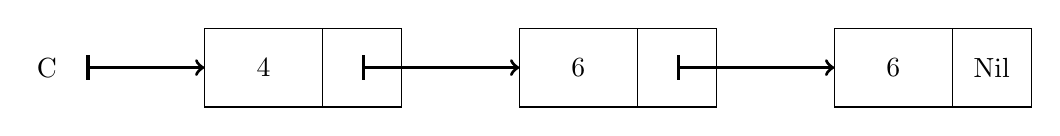
\begin{tikzpicture}
\node at(0,0.5){C};
\draw [very thick][|->](0.5,0.5)--(2,0.5);
\draw (2,0) rectangle(3.5,1);
\draw (3.5,0) rectangle(4.5,1);
\draw [very thick] [|->] (4,0.5)--(6,0.5);
\node at(2.75,0.5){4};
\draw (6,0) rectangle(7.5,1);
\draw (7.5,0) rectangle(8.5,1);
\node at(6.75,0.5){6};
\draw [very thick][|->](8,0.5)--(10,0.5);
\draw (10,0) rectangle(11.5,1);
\draw (11.5,0) rectangle(12.5,1);
\node at(10.75,0.5){6};
\node at(12,0.5){Nil};
\end{tikzpicture}
\end{figure}
Figure \ref{fig:1} on page \pageref{fig:1} 
\clearpage
\section{Ex.  6}
\begin{figure}[hbtp]
\centering
\label{fig:2}
\includegraphics[scale=1]{lionpic}
\caption{Lion}
\end{figure}
Figure \ref{fig:2} on page \pageref{fig:2} 
\section{Ex.  8}
\begin{equation}
a)\hspace{0.3 cm}({x^n})^2 + y^{n + 1} = z^n
\end{equation}
\begin{center}
(b)\emph{The Johansson Brothers \& Son}
\end{center}
(c) .. end of a paragraph. \\
A new paragraph ...\\
\section{Ex.  9}
\begin{lstlisting}
int main()
{
    int i;
    puts("LateX Program!");
    
    for (i = 0; i < N; i++)
    {
        puts("Exercise 9");
    }

    return 0;
}
\end{lstlisting}
\section{Ex.  10}
\newcommand{\summation}[1]{$$\sum\limits_{i=0}^n #1_i$$}
\summation{\alpha}
\summation{\beta}
\section{Ex.  11}
\begin{thebibliography}{9}
\bibitem{cameron99}
P. J. Cameron, \emph{Permutations Groups}, Cambridge University Press, Cambridge, 1999.
\bibitem{morton97}
P. Morton'Periods of Maps on Irreducible Polynomials over Finite Field',
\emph{Finite Fields and their Applications (Finite Fields Appl.)}, vol. 3, p. 11-24, 1997. 
\end{thebibliography}
\end{center}
\end{document}



